To evaluate the noise-removing filters that we proposed, we need a different approach than the model evaluation method. In this case, we have to invent our own metric system and display the results. We thought of a simple but effective way to display the performance of each filter. In this method, we will find the average motion data for each frame, and we will compute the change rate per frame (CRPF). The unfiltered data, due to the noise, should have greater CRPF than the filtered motion data. Moreover, we will find the best parameters that each filter has for motion data, and afterward, we will compare its CRPF in a graph. In the figures below, we demonstrate the evaluation of the three filters that we use, butterworth, mean and gaussian.


\begin{figure}[htp]
    \centering
    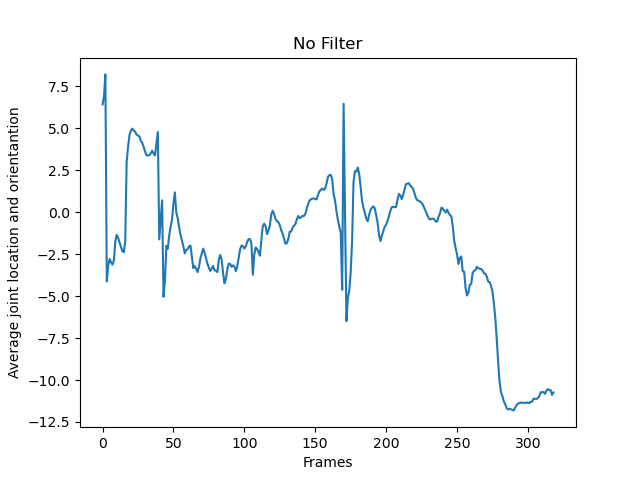
\includegraphics[width=0.45\textwidth]{figures/Evaluation/no_filter.png}%
    \qquad
    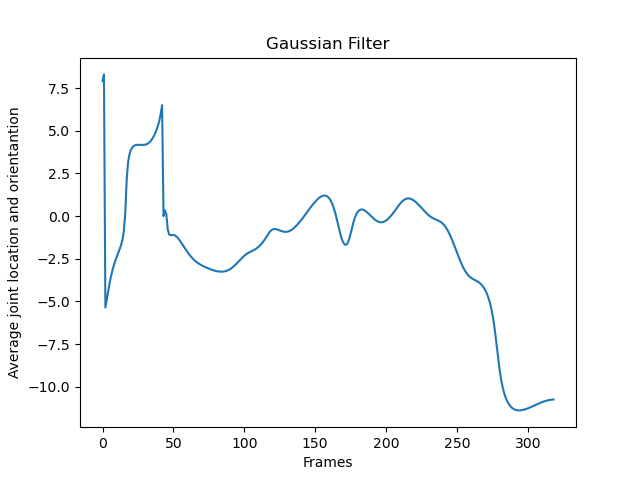
\includegraphics[width=0.45\textwidth]{figures/Evaluation/Gaussian_1000_3000.png}%
    \qquad
    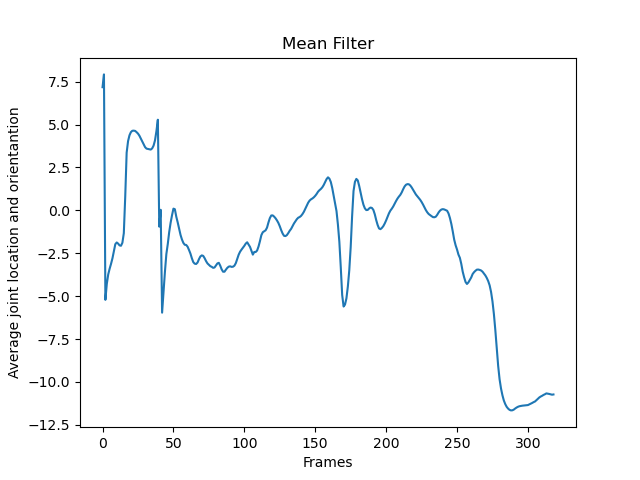
\includegraphics[width=0.45\textwidth]{figures/Evaluation/mean_7.png}%
    \qquad
    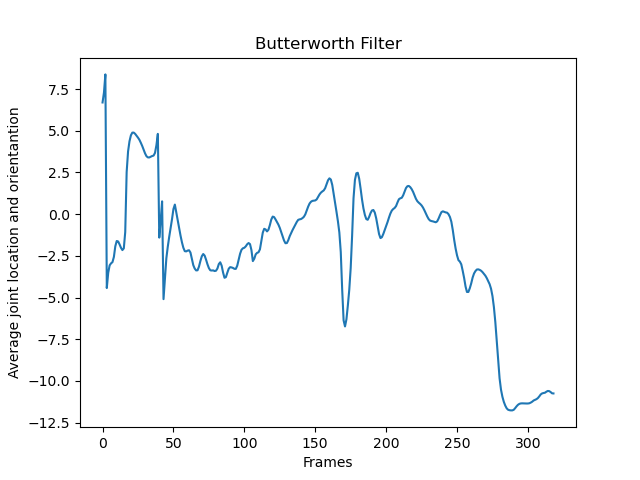
\includegraphics[width=0.45\textwidth]{figures/Evaluation/butterworth.png}%
    \captionsetup{labelformat=empty}
    \caption{Filtering comparison based on our metric system, CRPF}%
\end{figure}

In the above figure, we can clearly see that in the case that we do not use a filter, the motion data are too unstable between neighbor frames. This definitely means that these motion data contain noise. Regarding the filters, we can see that gaussian Filter has the smoothest graph. In addition, the results between the mean filter and the butterworth filter, are almost the same. At this point, it is worth saying that, we chose the best performance of each filter, which will remove the maximum amount of noise without affecting the motion data information.